\section{Verwandte Arbeiten}

\subsection{Arbeit 1}
\textcite{bazurto2019} beschäftigen sich mit sehr ähnliche Problemstellungen zu dieser Arbeit in Bezug auf den World Happiness Report. Sie stellen einen Mangel an Interaktivität und intuitiver Erforschung der Berichtdaten fest. Auch vergleichen sie dessen Visualisierungen mit denen des OECD Happiness Reports. Für diese Arbeit sind allerdings nur die Teile mit Bezug auf den World Happiness Report von Bedeutung. 

Sie setzen sich 6 Zielen, welche sie mittels Interaktiver Visualisierungen erreichen wollen. Diese Ziele Lauten:

\begin{itemize}
\item 1. Present the ranking, countries and their respective score

\item 2. Discover happiness distribution in the world. The user can interact with each country to obtain details on demand.
\item 3. Identify the happiness score and indexes by country

\item 4. Locate (knowing the country that I want to find (e.g. my country) a country and query how happy is it and how indexes are in this.

\item 5. Identify which countries are happier and which ones less happy extremes

\item 6. Discover happiness distribution in the different world regions. The user can interact with each country in those regions to obtain details on demand.
\end{itemize}

Hier ist viel Überschneidung mit den Zielen und Visualisierungen dieses Berichtes zu finden. Für die meisten dieser Ziele bietet auch dieser Bericht eine Antwort. Punkt 2,5 und 6 lassen sich durch den Scatterplot abdecken und 3 sowie 4 lassen sich durch eine Suche im Polarplot Dropdown beantworten. \\

Die Autoren entscheiden sich für insgesamt 5 Visualisierungen welche im Zusammenspiel diese Fragen beantworten sollen. Diese sind: Choroplethenkarte, Parallel Plot, Bar Chart, Ranking List sowie ein Bubble Chart. 
Die beste Vergleichsgrundlage bildet wohl Abbildung.\ref{fig:bazurto} , hier sind 
Die Choroplethenkarte, der Parallelplot und das Ranking enhalten. 
Wie bereits in der Schilderung der Visualisierungen erwähnt wäre der Parallelplot eine Alternative zum Polarplot gewesen. Hier ist der Unterschied deutlich zu sehen.
Es ist nun möglich die Dimensionen für alle Länder gleichzeitig darzustellen.\\

Die Authoren haben hier das Problem der Sichtbarkeit gut gelöst, indem sie das ausgewählte Land farblich hervorheben und die anderen Linien nur durch ein leichtes grau einzeichnen. Die anderen Linien tragen hier dennoch nicht viel Informationen bei, es lassen sich hier nicht wirklich zusätzliche Muster aus den Daten lesen das die Linen ineinander verschwinden.\\

Wirklich interessant und auch sehr intuitiv wirkt die Chloroplethenkarte. Hier lässt sich ein guter Überblick Über den Happiness-Score in der ganzen Welt gewinnen. Der Scatterplot ist nicht in der Lage die geographische Gruppierung so gut abzubilden wie eine Karte. Die Sublementierung mit der Regionenlegende ist nicht so Aussagekräftig. \\

\cite{bazurto2019}
\begin{figure}[h]
 \centering
 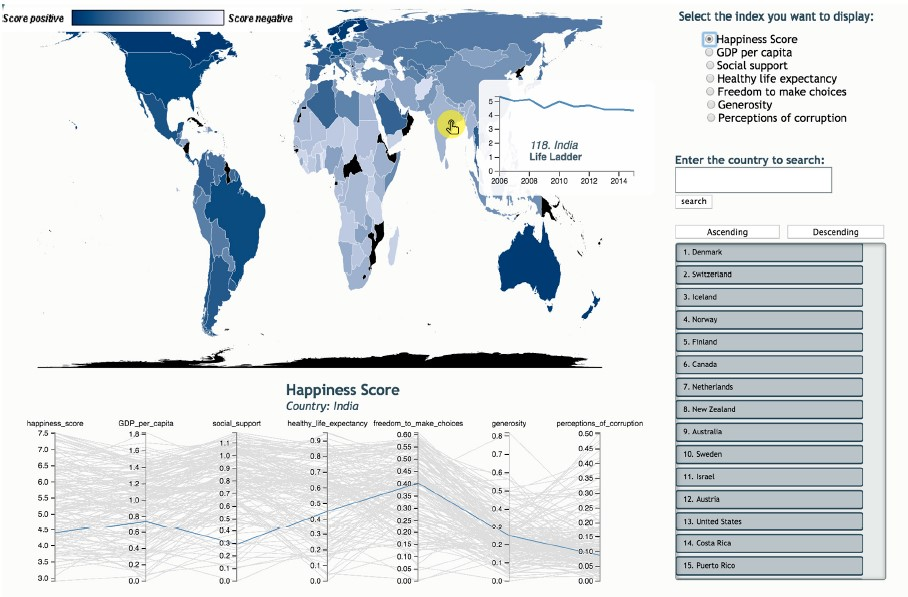
\includegraphics[width = 0.8\textwidth]{img/bazurto_vis.jpg}
 \caption{Visualisierung aus \textcite{bazurto2019}}
 \label{fig:bazurto}
\end{figure}

\subsection{Arbeit 2}

\textcite{happiness_2018} haben in ihrem Bericht \textit{Happiness Matters: An In-Depth Look into UN’s World Happiness Reports through Data Visualizations} mit den Daten aus dem World Happiness Report beschäftigt und wie diese am besten zu viualisieren sind. Ihre Daten behandeln den Zeitraum von 2015-2018. Die gesetzten Visualisierungsziele waren auch hier ähnlich genug um einen Vergleich zu ermöglichen. Die Ziele lauten: \\

\begin{itemize}
    \item 1. Identify the overall trends of happiness ranking index of different countries from 2015 to 2018
    \item 2. Identify the rankings of each of the 6 factors that make up the happiness rankings and how they are related to the final happiness rankings.
    \item 3. Compare the 6 factors between different countries from 2015 to 2018.
    \item 4. Compare different countries by geographical locations to find out the happiness patterns by regions.
\end{itemize}

\begin{figure}[h]
 \centering
 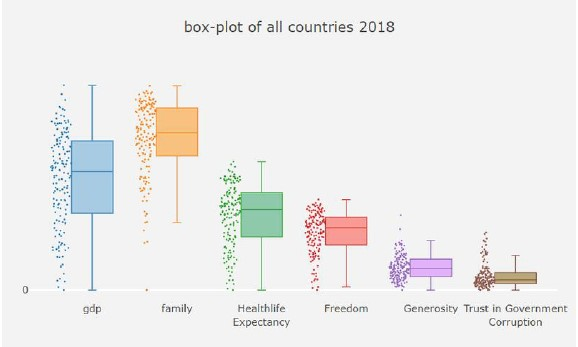
\includegraphics[width = 0.8\textwidth]{img/group12_boxplot.jpg}
 \caption{Boxplot aus \textcite{happiness_2018}}
 \label{fig:hap_2018}
\end{figure}

Eine interessante Visualisierungsmethode aus diesem Bericht ist in Abbildung.\ref{fig:hap_2018} zu sehen. Hier wurde eine Serie von Boxplots umgesetzt, einer für jeden Faktor. Besonders sind zudem die Punkteverteilungen welche neben den Boxplots abgebildet sind. Sie erleichtern es dem Nutzer die Verteilung noch etwas intuitiver wahrzunehmen. Außerdem lassen sich dort, wie auch im Scatterplot dieses Reports die Ländernamen anzeigen, wenn mit der Maus über den Punkten gehovert wird. \\

Eine Problem mit dieser Visualisierung ist die fehlende Achsenbeschriftung und nicht angepasste Skalierung für die einzelnen Dimensionen. So haben hier gdp und family den doppelten vertikalen Platz den Freedom einnimmt. Dies macht die kürzer dargestellten Variablen schlechter lesbar. Dies ist im Scatterplot dieser Arbeit besser erkennbar, dort ist die Skalierung variabel und es wird immer ein Maximum des Platzes im Graphen genutzt. Die Verteilung einer einzelnen Größe ist jedoch im Scatterplot nicht so deutlich zu verfolgen wie hier, da immer eine andere mit im Bild ist. 